
%-----------------------------------------------------
% Chapter 4: Descripción del prototipo
%-----------------------------------------------------
\chapter{Resultados: CoCADa Un software para el diseño colaborativo con LeanUX}
\label{cap:desarrollo}
\label{chap: cap3}

En este capítulo se implementa el proceso de \textit{Lean UX} en el desarrollo de CoCADa. El mismo se divide en cinco secciones, las cuatro primeras (\ref{vision-marco}, \ref{dis-des-colabo}, \ref{pmv-cocada} y \ref{feedback}) corresponden al uso de la metodología la cual describe las declaraciones, el diseño colaborativo, el desarrollo de los PMVs y experimentos y el \textit{feedback} con los usuarios. La última sección (\ref{sistema-cocada}) se enfoca exclusivamente a los aspectos técnicos del sistema tales como la arquitectura de software y las tecnologías involucradas.


\vspace{5mm}
\section{Declaraciones}
\label{vision-marco}
\textbf{Declaración del problema para CoCADa}:\vskip
\textquote{Los proyectos de diseños de productos son desarrollados por equipos de trabajo generalmente conformados por personas con diferentes competencias (profesiones o grados de conocimiento). Los participantes requieren comunicar sus ideas, proponer cambios y comprender la evolución de los productos, para ello es fundamental una comunicación eficiente. 
Se ha observado que las herramientas de comunicación más utilizadas en la actualidad (email, redes sociales, etc.) \textbf{dificultan la organización de los mensajes y la gestión de información sobre los proyectos}.
Esto genera problemas de interpretación de las características de los productos y dificulta el control sobre el trabajo realizado. En consecuencia, los participantes manifiestan una experiencia negativa durante el proceso, reduciendo su participación.

¿Cómo se podría mejorar la comunicación de modo que los que usuarios aumenten la colaboración de una manera ordenada y precisa?}

%\textquote{[El servicio/producto] debe cumplir con [estos objetivos]. Sin embargo, se ha observado que no se están alcanzando [estos objetivos], lo que está causando [este efecto adverso] para los usuarios. ¿Cómo se podría mejorar el  [servicio/producto] de modo que los usuarios consigan mejorar sus resultado según [estos criterios cuantificables o cualificables]?}\vskip

\vskip
%Evidentemente, esta declaración está repletas de suposiciones, para extraerlas se utiliza la siguiente lista u \textbf{hoja de suposiciones}.
Las \textbf{suposiciones} del problema son entonces las siguientes:


\begin{enumerate}

%\textbf{Hoja de suposiciones}:\vskip
\item\textbf{¿Quiénes son los usuarios del producto?}
\begin{enumerate}
\item \textbf{Personas sin conocimientos específicos}.
Interesados en participar del proceso de diseño sin tener conocimientos sobre diseño 3D. Generalmente solicitan modelos 3D para la visualización o para la fabricación digital. Estas personas pueden ser emprendedores, artistas, docentes, etc.

\item \textbf{Profesionales encargados de crear diseños 3D}. 
Poseen las capacidades técnicas y la experiencia sobre procesos y metodologías para llevar a cabo proyectos de diseño de productos.

\end{enumerate}

\item{\textbf{¿Cómo cambiaría el producto su trabajo?}}

\begin{enumerate}
    \item Ahorraría mucho tiempo en el  \textit{feedback}.
    \item De forma positiva, ya que es indispensable la organización en los cambios de los diseños.\vskip
\end{enumerate}

\item{\textbf{¿Qué problemas soluciona el producto?}}
    \begin{enumerate}
       \item La imposibilidad de visualizar el estado actual de un diseño. \vskip
       \item La comunicación inexacta a la hora de discutir sobre un producto.\vskip
    \end{enumerate}

    \item{\textbf{¿Cuáles serían las funciones más importantes?}}
    \begin{enumerate}
        \item Visualizar el modelo 3D de un producto.
        \item Comunicarse con el Diseñador de forma similar a un chat.
    \end{enumerate}

    \item{\textbf{¿Qué aspectos debe tener el producto y cómo debe comportarse?}}
    \begin{enumerate}
    \item Debe ser agradable a la vista, intuitivo y fácil de usar como una red social.
    \end{enumerate}
\end{enumerate}

\subsection{Hipótesis}
Desarrollando una herramienta de comunicación para proyectos de diseño de productos, se logrará una mayor colaboración en los equipos de trabajo. % que conforman los equipos de trabajo. 
Se sabrá si el desarrollo es correcto cuando aumente la participación entre las personas con diferentes competencias y se generen las condiciones necesarias para el co-diseño.

\subsection{Personas}
\label{personas}
En la figura \ref{fig:persona1} se analizan dos arquetipos que representan los dos tipos de usuarios del sistema. El usuario sin conocimientos de CAD (\textbf{Persona A}). El usuario profesional (\textbf{Persona B}).

\begin{figure}[ht]
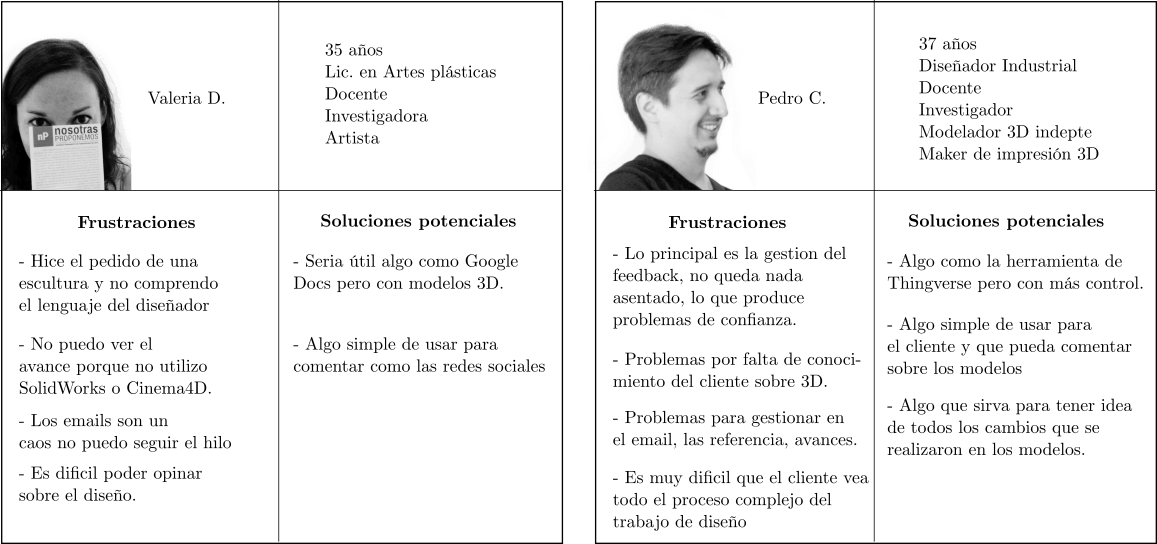
\includegraphics[width=16cm]{Img/Desarrollo/persona1.png}
\centering
\caption{\footnotesize{Personas utilizadas en CoCADa. El usuario sin conocimientos de CAD (Persona A)(izquierda). Usuario profesional (Persona B)(derecha). En la parte superior se especifica la información general del usuario. El cuadrante inferior izquierdo debe contiene las necesidades y  frustraciones respecto la solución actual, los puntos de conflicto específicos que el producto intenta resolver y/o la oportunidad que se trata de capturar con él. El cuadrante inferior derecho contiene las soluciones potenciales, sugeridas por el usuario.}}
\label{fig:persona1}
\end{figure}

\clearpage
\subsection{Funciones o funcionalidades}
\label{section:subhipo}
Con todo el material obtenido se organizan a continuación las sub-hipótesis que deben probarse. 

\begin{longtable}{|p{1cm}|p{4cm}|p{4cm}|p{4cm}| }

\hline
    Núm. & Se desarrolla (función) & Para (persona)  & Para (solución)\\
\hline
1 & Un visor de modelos 3D en la web & Para (Persona A) y  (Persona B) & Solucionar de forma eficiente la visualización de los productos \\

\hline
2 & Un sistema de comentarios asociado a los modelos 3D & Para (Persona A) y (Persona B)  & Discutir sobre los avances del proyecto.
\\

\hline
3 & Un mecanismo para anotaciones sobre los modelos 3D & Para (Persona A)  y (Persona B) & 
Poder comunicar aspectos de diseño entre personas de diferentes disciplinas  \\

\hline
4 & Un sistema para dar de Alta proyectos & Para (Persona B) & Gestionar nuevos proyectos de diseño.
\\

\hline
5 & Un mecanismo para escribir código de modelado & Para (Persona B) & Incorporar diseños y modificarlos mediante scripting \\
\hline
6 & Un mecanismo para ver los cambios o ``versiones" de los diseños & Para (Persona A) y (Persona B) & Visualizar la evolución de los modelos y su estado en una fecha determinada  \\
\hline

7 & Componentes visuales para modificar los parámetros del modelo 3D & Para (Persona A) y (Persona B) & Modificar geometrías de forma intuitiva, sin necesidad de tener conocimientos de programación o de modelado avanzado  \\

\hline
8 & Un mecanismo para inicio de sesión con usuario y contraseña & Para (Persona A) y (Persona B) & El ingreso privado  \\
\hline

\end{longtable}

\begin{center}
 \caption{\footnotesize{Tabla de sub-hipótesis para CoCADa}}
\end{center}

\clearpage
\section{Diseño Colaborativo}
\label{dis-des-colabo}
 
\begin{figure}[ht]
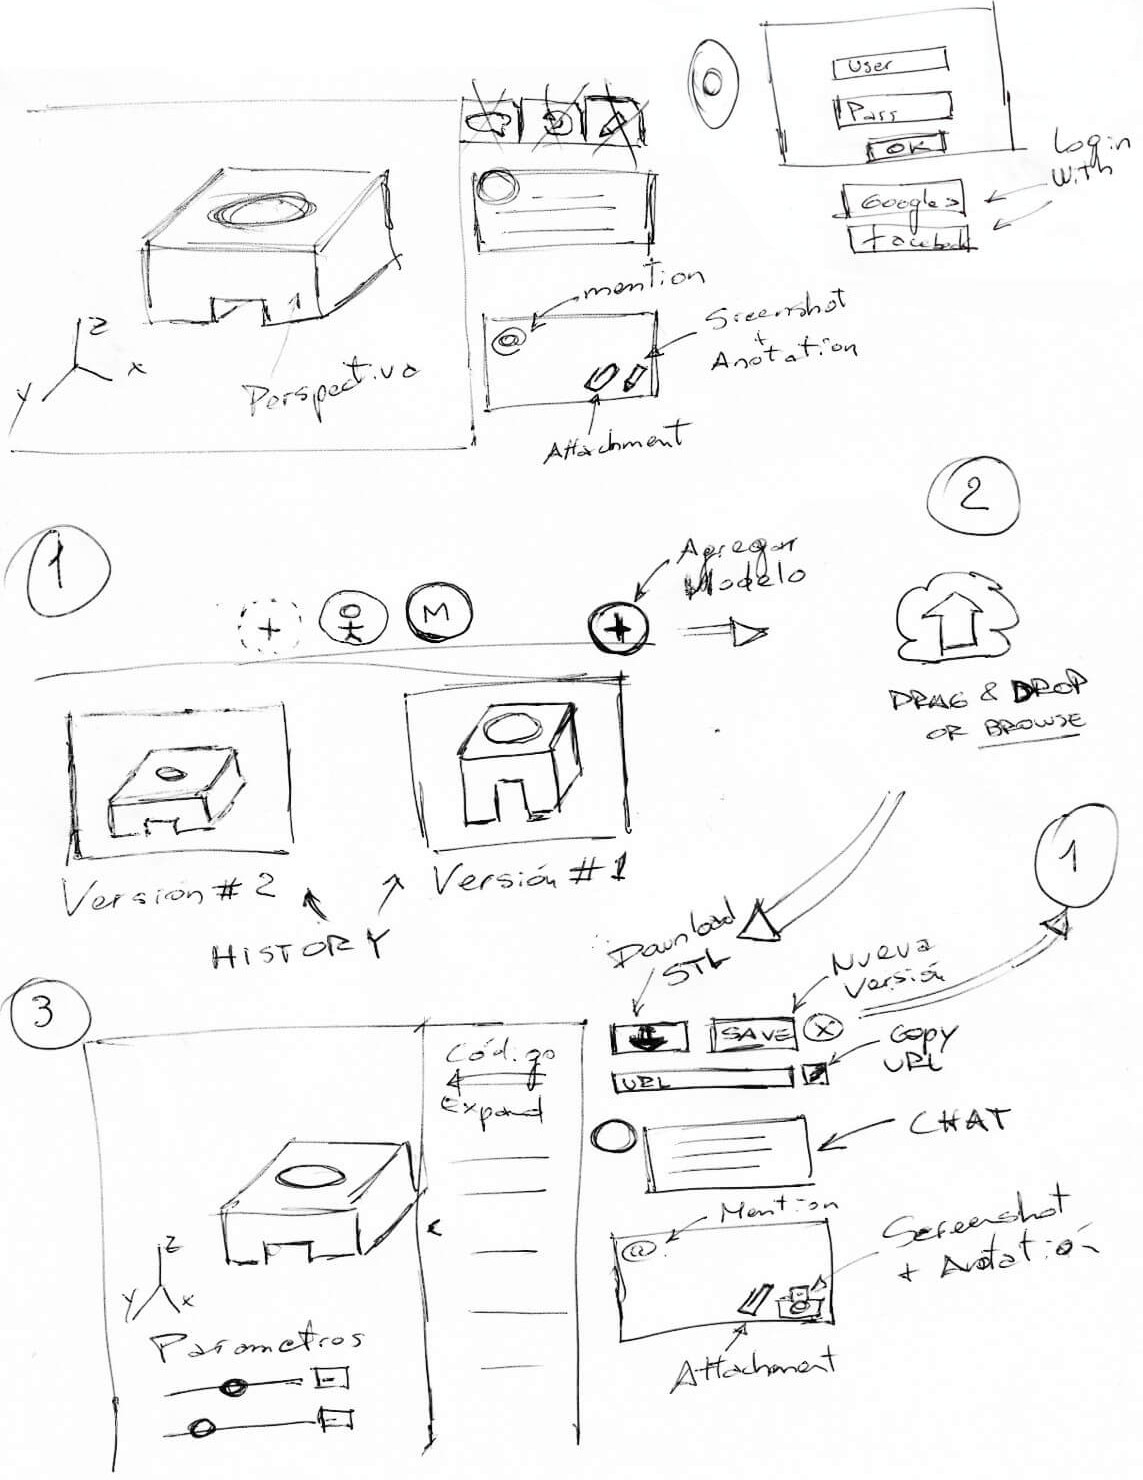
\includegraphics[width=7cm]{Img/UX/edc.jpg}
\centering
\caption{\footnotesize{Resultado del estudio de diseño explicado en la sección \ref{dis-colabo}. Sketchs o bocetos de interfaces de usuario para CoCADa.}}
\label{salida}
\end{figure}

\begin{figure}[ht]
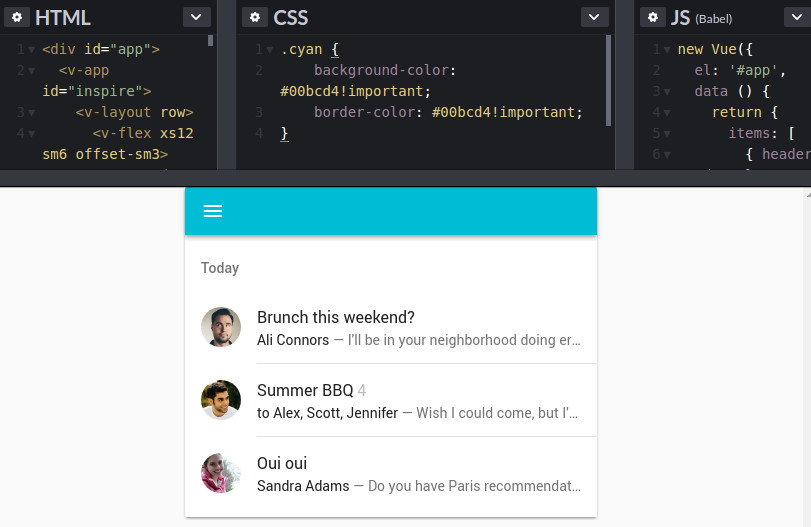
\includegraphics[width=8cm]{Img/Desarrollo/vuety.jpg}
\centering
\caption{\footnotesize{Guía de estilo utilizada en CoCADa. Ejemplo de componente web para conversaciones y su forma de uso mediante código HTML, CSS y javascript.}}
\label{vuetify}
\end{figure}


\clearpage
\section{PMV y experimentos}
\label{pmv-cocada}

El primer PMV o \textbf{Demo \#1} evaluó la \textbf{sub-hipótesis 1} de la tabla de sub-hipótesis: ``\textbf{Un visor de modelos 3D en la web para el usuario (Persona A) y (Persona B) para solucionar de forma eficiente la visualización de los productos}''.\vskip
Se utilizaron tres preguntas para orientar el experimento: 
\begin{enumerate}
    \item \textbf{¿Quién interactuará efectivamente con el prototipo?} \\
    El usuario sin conocimientos de CAD (Persona A).
    \item \textbf{¿Qué se espera aprender de él?} \\
    Aspectos de funcionalidad y usabilidad de la interfaz UI al  momento de interactuar con un modelo 3D.
    \item \textbf{¿Cuánto tiempo se tiene para desarrollar el prototipo?}\\ Aproximadamente 4 días.
\end{enumerate}

Se utilizaron \textbf{prototipos de alta fidelidad} \citep{Gamble2016} %\textquote{\textit{La fidelidad se refiere al nivel de realismo en un prototipo}} . 
para lograr un aspecto y comportamiento similar al de la interfaz definitiva.

En el primer experimento se presentó un prototipo de visor con un modelo 3D (ver figura \ref{fig:feedback0})  %y funcionalidades de zoom (alejar, acercar), rotación y traslación. También se presentan los parámetros para modificar la geometría y el color 
, programado en base 
al código de OpenJSCAD en un tiempo aproximado de 36 horas.

\begin{figure}[ht]
    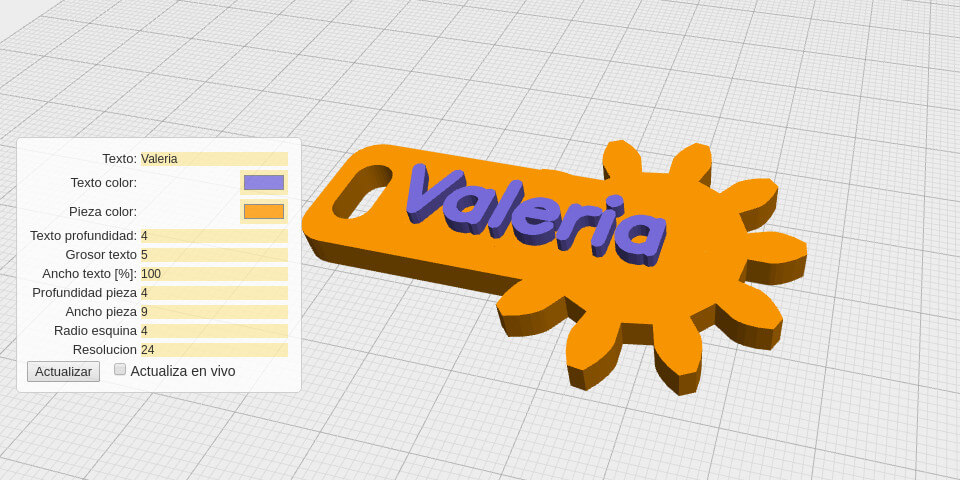
\includegraphics[width=14cm]{Img/Desarrollo/feedback0.jpg}
    \centering
    \caption{\footnotesize{Pantalla  de Demo \#1. Visor con un modelo 3D (centro) y funcionalidades de zoom (alejar, acercar), rotación y traslación. Parámetros para modificar la geometría y el color (izquierda).}}
     \label{fig:feedback0}
\end{figure}


\subsubsection{Características del experimento:} 
Se utilizó una computadora con conexión a internet y un navegador web mostrando el modelo por defecto en la pantalla. El usuario no recibió instrucciones sobre el uso y no tiene limitaciones de tiempo. El evaluador se limitó a observar y registrar la actividad.

\section{Feedback}
\label{feedback}

Al final de la sesión de prueba se realizaron una serie de preguntas sobre la experiencia de usuario, divididas en tópicos. \\ 
Las respuestas posibles fueron: \textbf{Buena, Regular o Mala}. En caso de responder Regular o Mala se realizaron otras 2 preguntas: \textbf{¿Cuál es el inconveniente?} y \textbf{¿Qué sugiere para resolver ese inconveniente?}\\ 
En la siguiente tabla se detallan los tópicos y sus respuestas:

\begin{longtable}{ |p{0.8cm}|p{2.3cm}|p{2.2cm}|p{3.6cm}|p{3.6cm}| }
\hline
     Ítem & Tópico & Experiencia  & Inconveniente & Cómo mejorar\\
\hline
1 & Visualización del Modelo & Buena & - & -\\
\hline
2 & Zoom & Regular & Al hacer demasiado zoom sobre el modelo ocurre que no hay un limite, lo que produce que se rompa la geometría. & Limitar el zoom o ver la posibilidad de volver la visualización a su estado original.
\\
\hline
2 & Rotación & Buena & - & -\\
\hline
3 & Translación & Mala & Al mover demasiado el modelo, ocurre que se pierde la visualización y parece que la escena esta vacía. & Limitar la opción de mover o ver la posibilidad de volver la visualización a su estado original.
\\
\hline
4 & Modificación de parámetros & Regular & Es incómodo ingresar números utilizando el teclado & Agregar un elemento parecido a los que tienen las apps.\\
\hline
\end{longtable}
\begin{center}
    \caption{\footnotesize{Resultados del feedback para Demo \#1}}
\end{center}

\subsection{Resultados y propuestas}
Luego de replicar y analizar las \textbf{experiencias de usuario negativas},  se construyó un prototipo \textbf{Demo \#2} en base al feedback y las recomendaciones del usuario en el experimento con Demo \#1.

\begin{itemize}

    \item \textbf{Zoom} (alejar, acercar). En la figura \ref{fig:feedback1} se puede apreciar como se ``rompe" la geometría. 
    %No se dispone de un mecanismo para la corrección.\vskip 
    \textbf{Solución}: Se agrega un botón de ``Resetear Vista'' (izquierda) para establecer la cámara en la posición original, con el objeto centrado en la pantalla (ver figura \ref{fig:feedback4} , izquierda).
    
    \begin{figure}[h]
    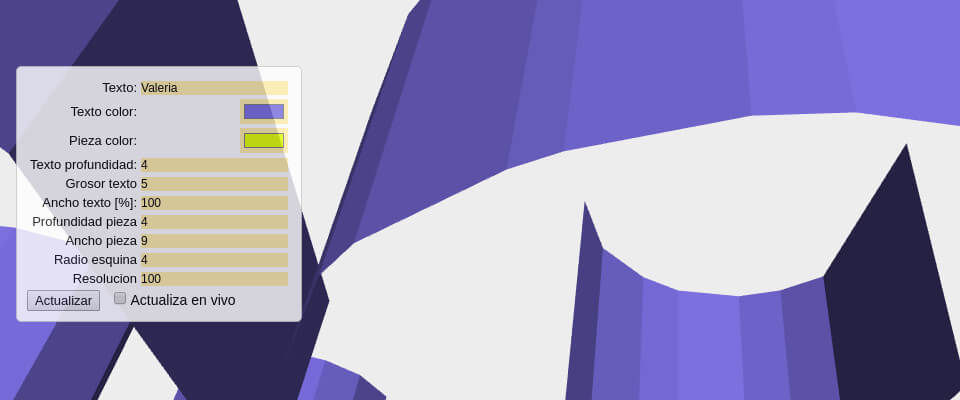
\includegraphics[width=14cm]{Img/Desarrollo/feedback2.jpg}
    \centering
    \caption{\footnotesize{Inconvenientes  con el zoom en Demo \#1. Se ``rompe'' la geometría.}}
     \label{fig:feedback1}
    \end{figure}
    
    \item \textbf{Traslación} (Mover). En la Figura \ref{fig:feedback2} el modelo prácticamente desaparece de la pantalla. %No existe un mecanismo para salir de esta situación. \vskip
    \textbf{Solución}: Se utiliza la misma funcionalidad de el punto anterior.
    
    \item \textbf{Modificación de parámetros}. La mayoría de las personas están acostumbrados a las interfaces con componente gráficos como deslizadores en los que no es necesario escribir  valores numéricos. Tanto en la figura \ref{fig:feedback1} como en la figura \ref{fig:feedback2}(izquierda) no se visualizan este tipo de elementos.\vskip 
    
    \textbf{Solución}: Se agrega un componente \textit{slider} como parámetro ``Texto profundidad" (ver figura \ref{fig:feedback4} , izquierda) para evitar la carga de valores numéricos por teclado. El resto de los campos de texto no se han modificado, intencionalmente, para que el usuario pueda evaluar las diferencias en el uso.

\end{itemize}


   \begin{figure}[h]
    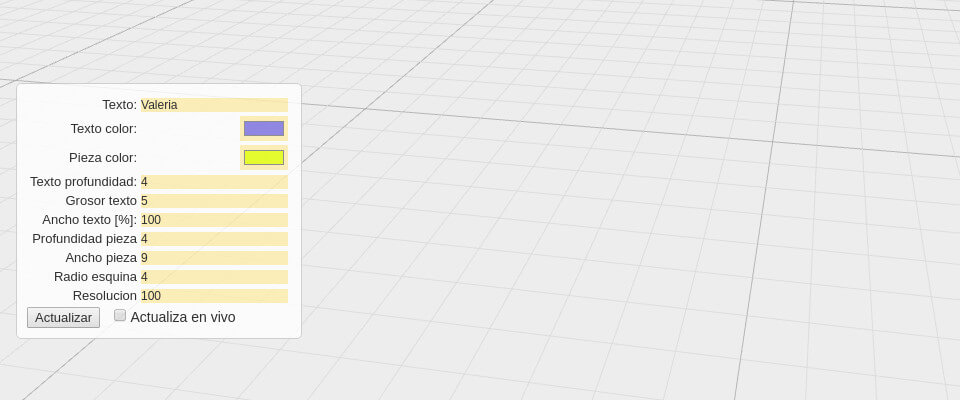
\includegraphics[width=14cm]{Img/Desarrollo/feedback3.jpg}
    \centering
    \caption{\footnotesize{Inconvenientes con la traslación en Demo \#1. El objeto se sitúa fuera del campo de visión. También se observan problemas con la modificación de parámetros (izquierda), el uso de campos de textos no es adecuado para valores numéricos.}}
     \label{fig:feedback2}
    \end{figure}


\begin{figure}[ht]
    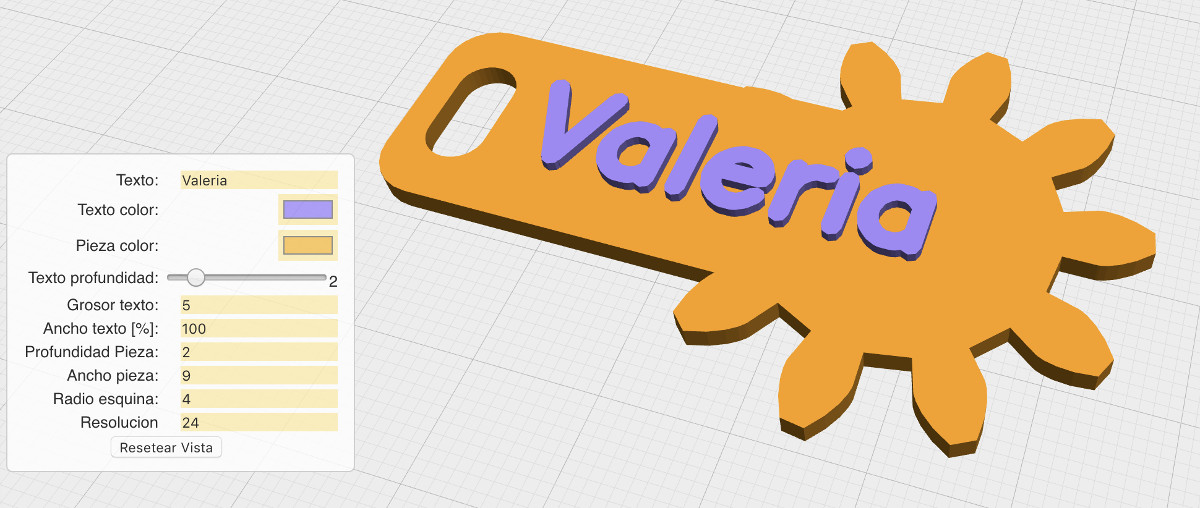
\includegraphics[width=14cm]{Img/Desarrollo/feedback4.jpg}
    \centering
    \caption{\footnotesize{Demo \#2. Corrección de inconvenientes hallados en Demo \#1. Se agrega un botón ``Resetear vista'' para solucionar el problema del zoom. Se agrega el componente ``slider'' como parámetro ``Texto profundidad'' para mejorar la experiencia de usuario al modificar los valores numéricos. }}
    \label{fig:feedback4}
\end{figure}

Al finalizar cada experimento se vuelve al ciclo \textit{construir-medir-aprender} visto en la sección \ref{section:pmv}, hasta obtener un prototipo que satisfaga al usuario. De esa manera se obtuvieron recomendaciones interesantes para ser implementadas en el futuro: en el experimento con Demo \#2, el usuario sugirió utilizar la funcionalidad de \textit{reset}\footnote{Reiniciar, en inglés \textit{reset} se conoce como la puesta en condiciones iniciales de un sistema.} pero en los parámetros y de forma individual, un requerimiento de la vista general adaptado a los componentes.\\
Con la tabla de sub-hipótesis y lo aprendido con el usuario en los experimentos, finalmente se estableció la arquitectura de software necesaria para dar soporte a todas las funcionalidades de CoCADa.

\clearpage
\section{Sistema CoCADa}
\label{sistema-cocada}

En la sección \ref{section:subhipo} se identificaron las  funcionalidades que la aplicación debe proveer a los usuarios. Adicionalmente, para una colaboración distribuida, se requiere de la \textbf{Gestión de datos de productos basado en la web} (WPDM), explicada en la sección \ref{sec:pdm}. CoCADa se divide en dos áreas fundamentales: \textit{Back-End} y \textit{Front-End} \citep{mardan2015full}.



    
\subsection{Back-End}
La aplicación de \textit{Back-End} o capa de servicios cuenta con tecnologías para tareas que no pueden ser resueltas directamente por los usuarios como la persistencia de datos y el almacenamiento de archivos. Las tecnologías utilizadas son:

\begin{itemize}

    \item \textbf{Node.js}\footnote{\url{https://nodejs.org/es/}} como web server y entorno de ejecución para JavaScript en el lado del servidor, de la misma manera que lo hacen otros lenguajes como PHP\footnote{\url{http://php.net/manual/es/intro-whatis.php}} o Python. 
    
    \item \textbf{Nuxt.js}\footnote{\url{https://nuxtjs.org/}}. Es un framework para crear aplicaciones isomórficas o universales con Vue.js\footnote{\url{https://vuejs.org/}}. Una aplicación  universal  es  aquella  que su código puede ser ejecutado tanto en el cliente (navegador web) como en el servidor. Nuxt.js incorpora el concepto \textit{Server Side Rendering}  (SSR)\footnote{\url{https://ssr.vuejs.org/#what-is-server-side-rendering-ssr}}.
    El SSR en CoCADa brinda la posibilidad de convertir los  componentes web en cadenas de HTML en el servidor, luego son enviadas al navegador web y se genera la aplicación en el lado del cliente. 
    
    \item \textbf{LoopBack}\footnote{\url{https://loopback.io}}. Es un conjunto de módulos de Node.js que permiten la implementación de APIs \citep{masse2011rest} altamente flexibles. Está basado en el framework \textbf{Express.js}\footnote{\url{https://expressjs.com/es/}} y proporciona funcionalidades para:
    
    - Crear APIs REST dinámicas end-to-end\footnote{End-to-end es un enfoque que involucra la visión global del encadenamiento de procesos y/o actividades, desde que surge una necesidad a satisfacer, hasta que esta es satisfecha} con poca codificación.\\
    - Acceso a datos para los principales motores de bases de datos, servicios SOAP y otras APIs. \\
    - Almacenamiento de archivos o \textit{file storage}.\\
    - Inicio de sesión mediante protocolos de autorización OAuth\footnote{\url{https://oauth.net/2/}}.\\
    Nuxt.js se comunica con LoopBack a través de su API REST , obteniendo como respuesta es un documento JSON.
    
    \item \textbf{MongoDB}\footnote{\url{https://www.mongodb.com/es}}. El enfoque de CoCADa es agnóstico\footnote{Se refiere a la capacidad de interoperabilidad y compatibilidad de un componente de cómputo entre diversos sistemas y ambientes, sin requerir una adaptación especial. } respecto al motor de base de datos, sin embargo, se utiliza MongoDB (NoSQL) para la persistencia de datos. A diferencia de las bases de datos relacionales, los datos se almacenan en tablas, sino mediante documentos en formato JSON. Esto permite que la integración entre MongoDB y javascript sea mucho más directa.

\vskip
\end{itemize}

\begin{figure}[h]
    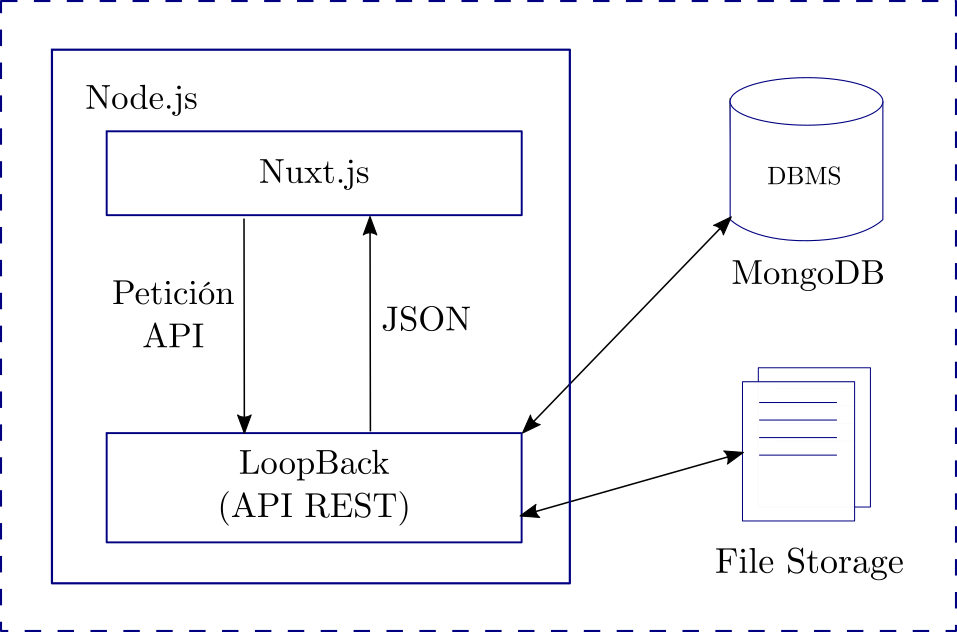
\includegraphics[width=8cm]{Img/Desarrollo/backendf.png}
    \centering
    \caption{\footnotesize{Backend de CoCADa. Node.js se utiliza como web server y entorno de ejecución para JavaScript. Nuxt.js provee el Server Side Rendering (SSR). Loopback implementa la API REST y gestiona los archivos (File Storage). MongoDB es el motor de bases de datos. Nuxt.js se comunica con LoopBack a través de su API, obteniendo como respuesta un documento JSON.}}
     \label{fig:sistema0}
\end{figure}

\subsubsection{CoCADa API REST}
En esta sección se desarrolla el modelo lógico del sistema, incluyendo el soporte para \textbf{Intercambio de datos Basado en Características} (FBDE) explicado en la sección \ref{FBDE}. El diagrama de la figura \ref{fig:schema} ilustra el esquema de datos y las relaciones entre las entidades. Las especificaciones del modelo y la fuentes de datos (base de datos) se realizan con LoopBack mediante archivos JSON.



\begin{figure}[h]
    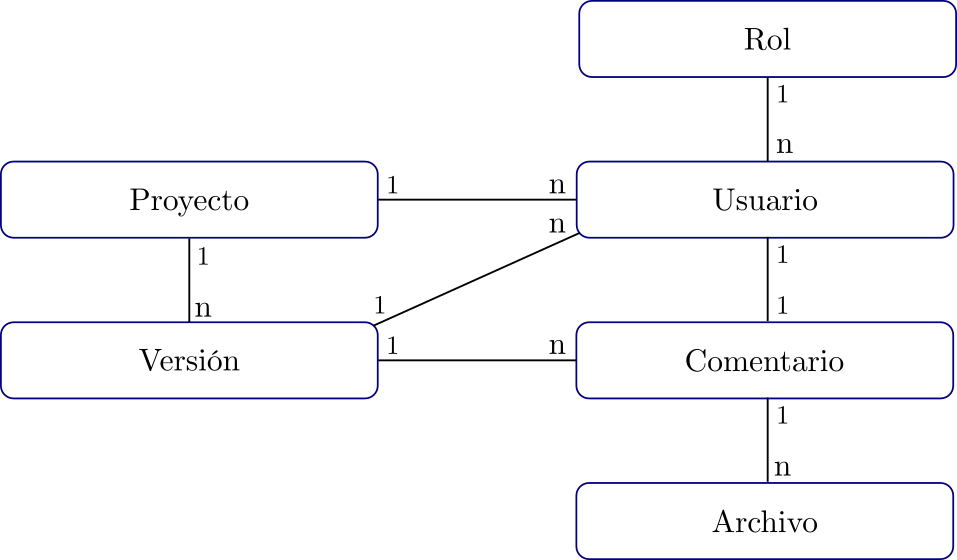
\includegraphics[width=10cm]{Img/Desarrollo/cocada-de0.png}
    \centering
    \caption{Modelo de datos para CoCADa. Un Proyecto puede contener versiones de un producto (árbol de historias). Una Versión puede ser utilizada por uno o más usuarios en el marco de trabajo, también soporta conversaciones de estos usuarios a través de Comentarios. Un Usuario puede asumir un rol específico. Un Comentario puede contener uno o más archivos. }
    \label{fig:schema}
\end{figure}

\begin{itemize}
    \item \textbf{Proyecto}: Es la entidad que gestiona la  evolución de los diseños. Puede contener una o más versiones de un producto, también llamado árbol de historias (ver figura \ref{fig:schema}). 
    
    En la figura \ref{fig:schema2} se puede analizar un  proyecto con su respectivas versiones y la evolución de los diseños.
    \begin{figure}[h]
    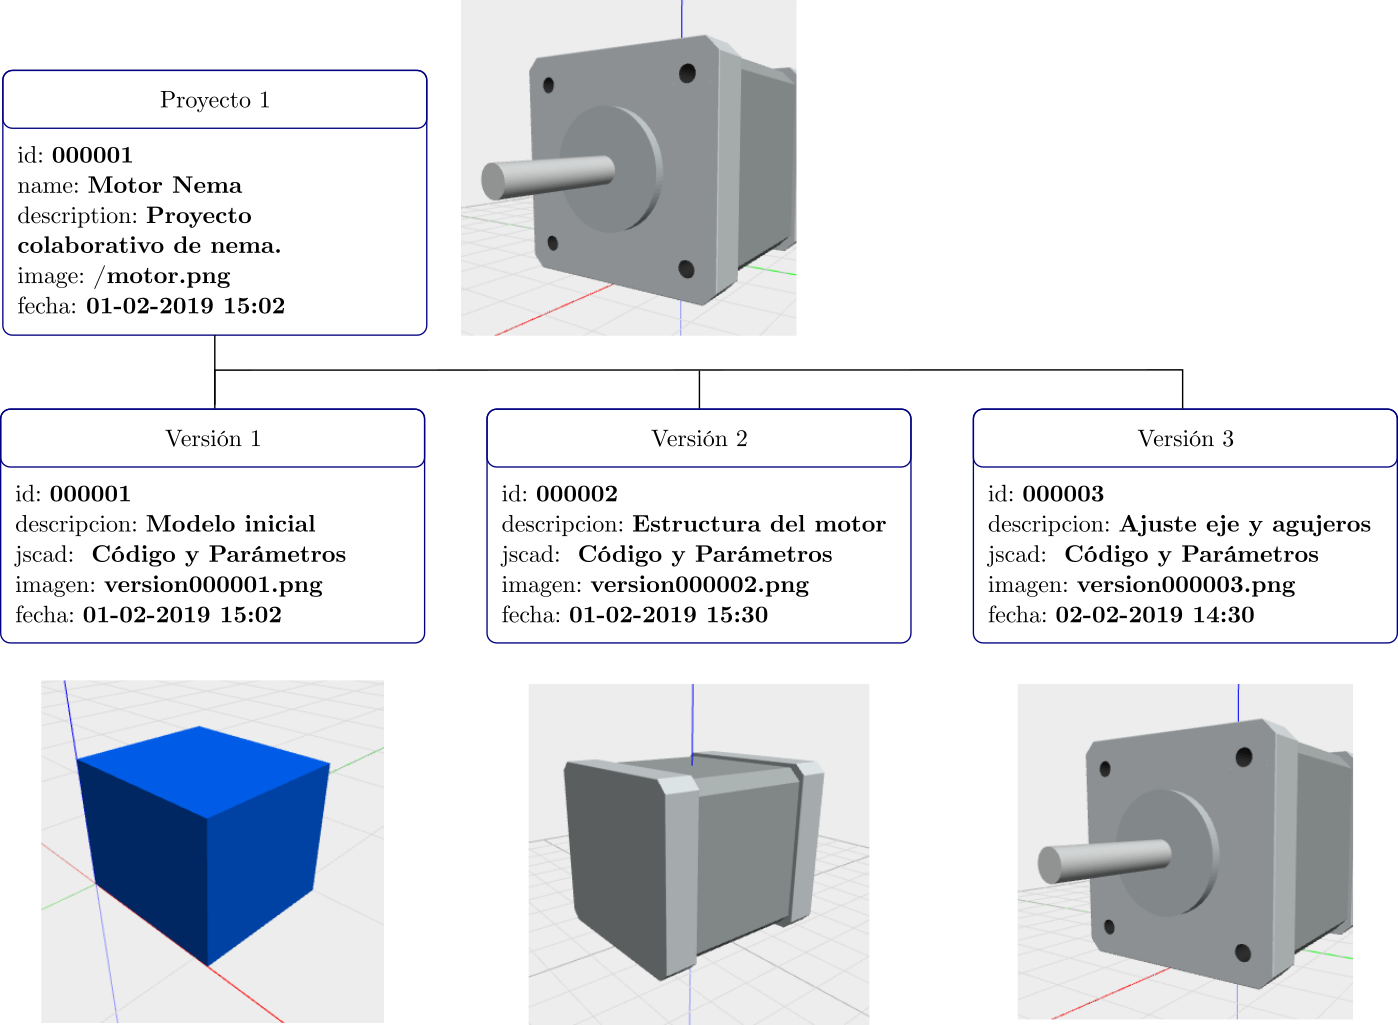
\includegraphics[width=16cm]{Img/Desarrollo/cocada-de.png}
    \centering
    \caption{\footnotesize{Un proyecto con su árbol de historia o versiones. Se puede apreciar la evolución del producto ordenada por fecha ascendente. La imagen que identifica el $Proyecto \ 1$ es la misma que la última versión del producto. La $Versión \ 1$ se inicia al momento de generar el proyecto, con un modelo de ejemplo (cubo). La $Versión \ 2$ se genera a partir de la anterior, con los cambios efectuados en el código y así sucesivamente.}}
    \label{fig:schema2}
    \end{figure}
    
    \item \textbf{Versión}: Es la representación de un diseño (producto) individual y su información relacionada. También se puede entender como una iteración en el proceso de diseño. 
    
    
    \item \textbf{Usuario}. La entidad representa a los usuarios del sistema. 
    
    \item \textbf{Comentario}. 
    Es la entidad que gestiona los comentarios asociados a una Versión.
    
    \item \textbf{Rol}. Especifica los permisos de los usuarios dentro del sistema, un mismo rol puede ser asignado a diferentes usuarios.
    
    \item \textbf{Archivo}. Esta entidad contiene la dirección web o URL de un archivo, en CoCADa estos archivos se asocian a los comentarios.
    
\end{itemize}

Para facilitar el desarrollo, LoopBack provee una herramienta (\textit{API Explorer}\footnote{\url{https://loopback.io/doc/en/lb3/Use-API-Explorer.html}}) para explorar las entidades, los metodos HTTP disponibles y los \textit{EndPoints}\footnote{Un Endpoint en la API de CoCADa es una URL única que representa un objeto o una colección de objetos.} de la API. En la figura \ref{fig:explorer} se puede ver un modelo ``Versión'' utilizado como prueba.

\begin{figure}[ht]
    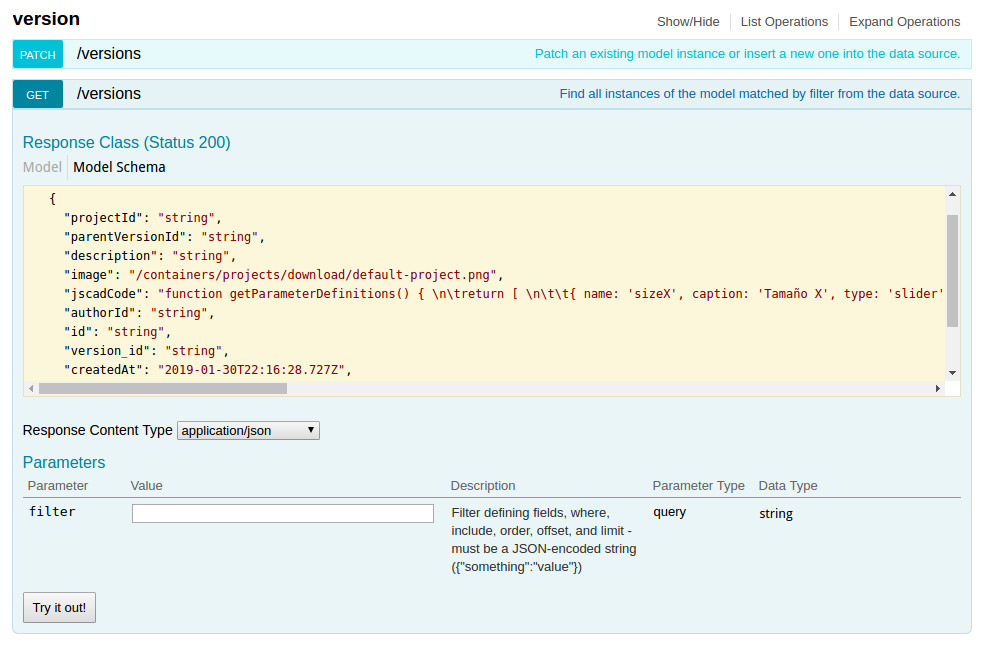
\includegraphics[width=16cm]{Img/Desarrollo/strong.jpg}
    \centering
    \caption{\footnotesize{Herramienta API Explorer de LoopBack. Se muestra el contenido de un modelo ``Versión'', se pueden apreciar los datos del producto.}}
    \label{fig:explorer}
\end{figure}

\clearpage
\subsection{Front-End}
\label{front}
En las aplicaciones web, el \textit{Front-End} o capa de presentación implica el uso de las tecnologías con las que interactúa directamente el usuario. Normalmente estas tecnologías son desarrolladas en los lenguajes HTML, CSS, javacript y otros recursos como imágenes y gráficos vectoriales (ver figura \ref{fig:front}). Al ingresar al sistema, se muestra la interfaz de usuario UI también llamada CoCADa APP.

\begin{figure}[h]
    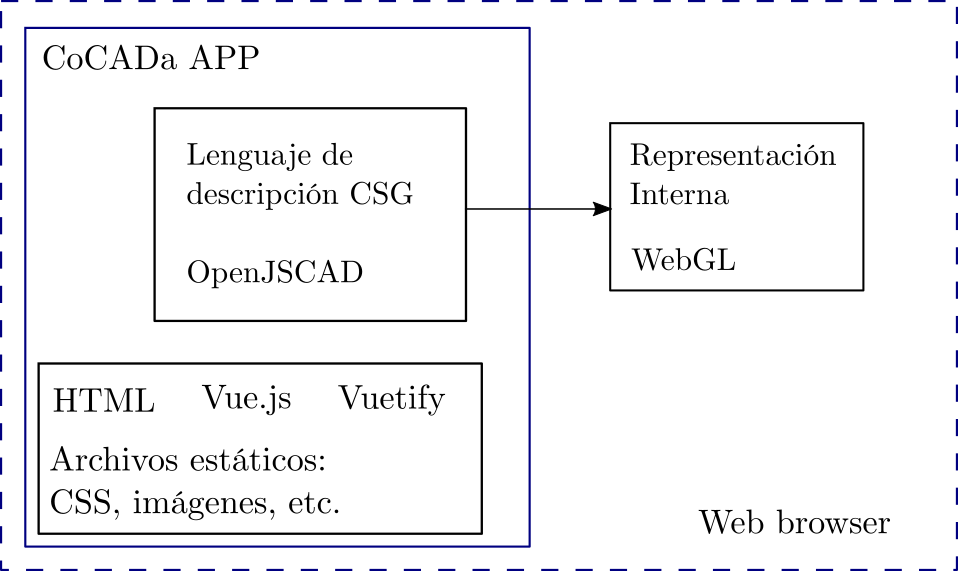
\includegraphics[width=10cm]{Img/Desarrollo/front.png}
    \centering
    \caption{\footnotesize{Frontend de CoCADa. CoCADa APP está compuesta por OpenJSCAD (Lenguaje de descripción) y Vue.js como sistema reactivo + Vuetify (Material Design). WebGL resuelve la representación interna (matemática) en el navegador web.}}
    \label{fig:front}
\end{figure}

Para la implementación se utilizan las siguientes tecnologías:
\begin{itemize}

     \item \textbf{OpenJSCAD} (javascript) como \textbf{lenguaje de descripción CSG} para trabajar en alto nivel y de forma intuitiva con las primitivas, transformaciones, operaciones booleanas, etc. Además provee mecanismos para la manipulación visual de parámetros y exportación de los modelos en formato STL. Una vez procesadas las sentencias del lenguaje de descripción, se traducen a su  \textbf{representación interna} (matemática) vista en la sección \ref{repGeo} mediante la API \textbf{WebGL} del navegador web (ver figura \ref{fig:front}).
     
    \item \textbf{Vue.js}\footnote{\url{https://vuejs.org/}}. Es un framework progresivo para interfaces de usuario, lo que significa que se pueden incorporar herramientas incrementalmente, a medida que aumenta la complejidad de la aplicación. Un ventaja de usar esta tecnología es su característica de sistema \textbf{reactivo} \citep{mezzalira2018front}, manteniendo una interacción constante con su entorno y permitiendo el cambio de estado interno por medio de eventos. 
    Cuando los datos de la interfaz son modificados por alguna acción del sistema o del usuario, por ejemplo: cada vez que se hace una petición al \textit{Back-End} (ver figura \ref{fig:front-backend}), tiene la capacidad de modificar solamente los componentes necesarios, sin necesidad de actualizar toda la aplicación en el navegador web.
    
    \item \textbf{Vuetify}\footnote{\url{https://vuetifyjs.com/en/}}.  Es un framework progresivo orientado a componentes visuales, se basa en el concepto \textit{Material Design}\footnote{\url{https://material.io/design/}}, con elementos reconocibles por los usuarios en la mayoría de las apps. Se utiliza para lograr una experiencia de usuario satisfactoria, en base al diseño establecido en la sección \ref{dis-des-colabo}.\vskip
    
   

\end{itemize}


Para una mejor comprensión de la UI, se hace una  distinción entre pantallas y componentes.


\subsubsection{Pantalla de Proyectos}
Luego del \textit{login} mediante un usuario y contraseña, se muestra una pantalla con el listado de proyectos (ver figura \ref{fig:cocada1})(izquierda).

\begin{figure}[h]
    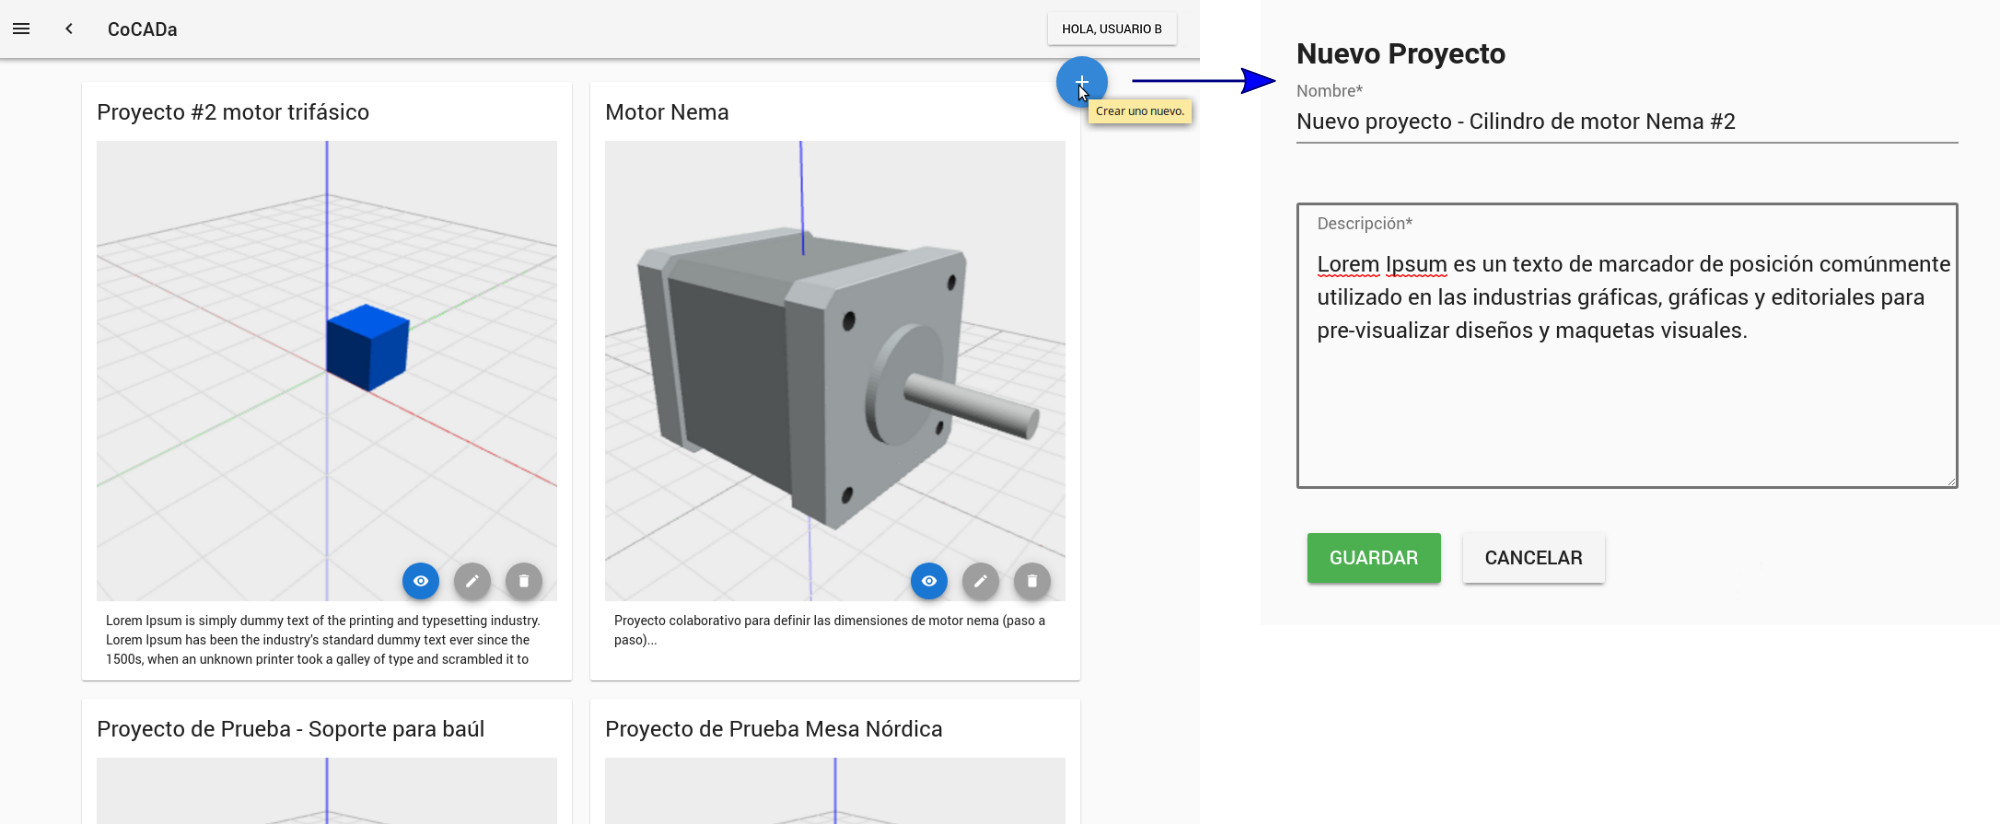
\includegraphics[width=16cm]{Img/Desarrollo/cocada0.jpg}
    \centering
    \caption{\footnotesize{Pantalla de proyectos (izquierda), en primera instancia se muestra un listado de proyectos con la posibilidad de ver, editar y eliminar los mismos. Al hacer click en la llamada a la acción (botón) en la parte superior derecha de la ventana se agrega un nuevo proyecto. A la derecha se puede observar el formulario de alta para un nuevo proyecto. Los usuarios Persona A y Persona B pueden agregar proyectos.}}
     \label{fig:cocada1}
\end{figure}

\subsubsection{Pantalla de Producto}
Un producto se refiere a una versión especifica del mismo dentro del árbol de historia. 
Al agregar un nuevo producto o al ``ver'' un proyecto del listado, se muestra la pantalla de la figura \ref{fig:cocada2}, correspondiente a la vista de producto. 

\begin{figure}[ht]
    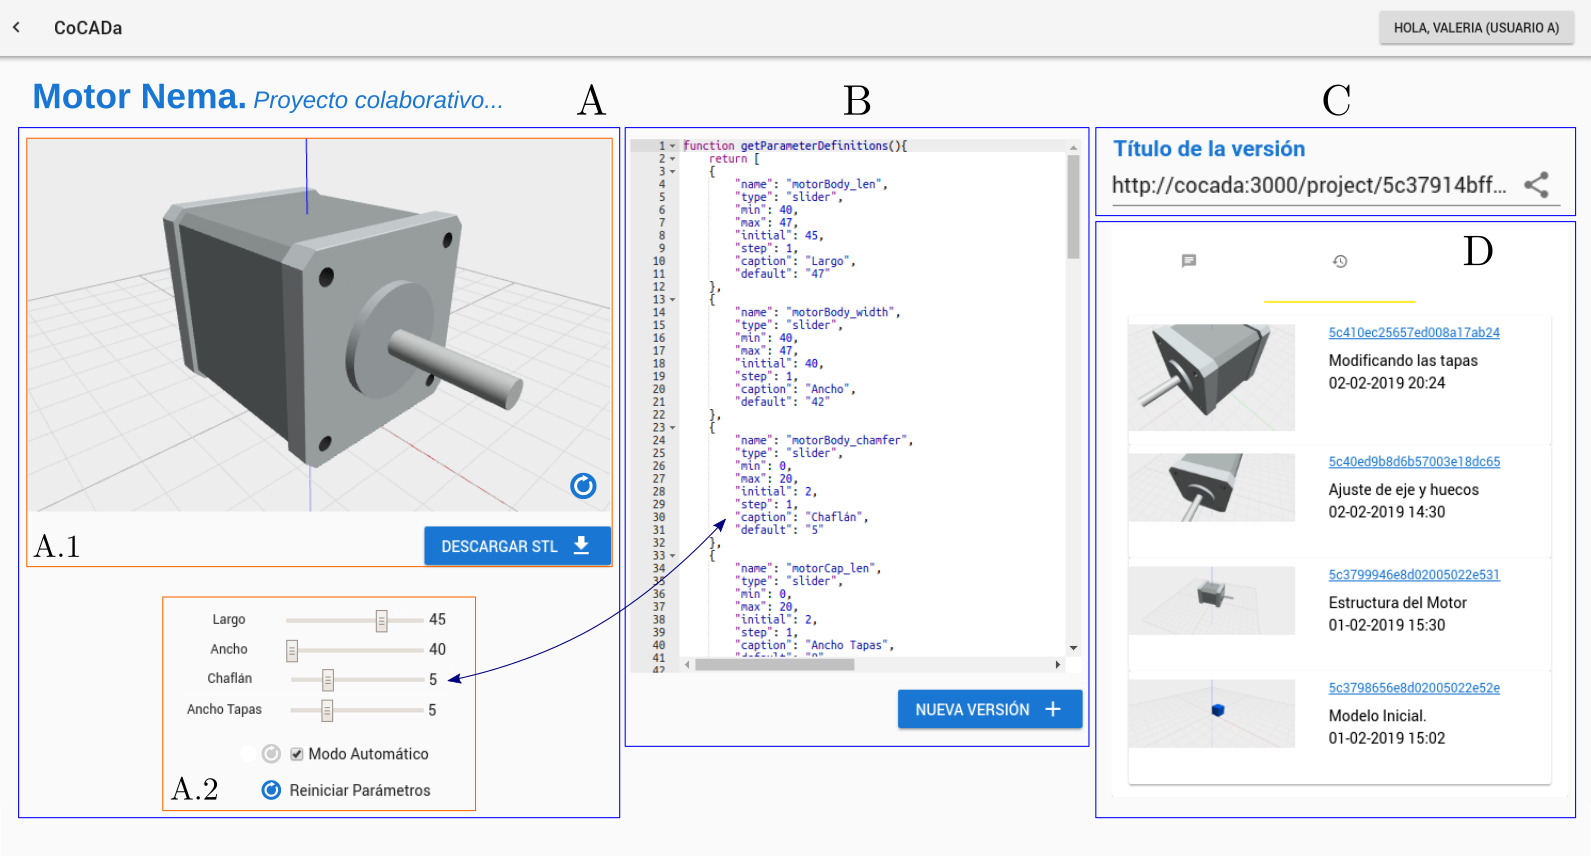
\includegraphics[width=16cm]{Img/Desarrollo/cocada-pantalla.png}
    \centering
    \caption{\footnotesize{Pantalla de Producto. Visor 3D (A) (izquierda). Editor de código (B) (centro). Componente para compartir el modelo (C) (derecha y arriba). Componente de comentarios e historial de modelos (D) (derecha y abajo).}}
     \label{fig:cocada2}
\end{figure}

Los componentes web de la pantalla son:
\begin{itemize}
\item \textbf{A. Componente del Visor 3D} (izquierda). \\


\begin{itemize}
\textbf{A1. Modelo 3D}. Se visualiza el modelo mediante OpenJSCAD y WebGL. Funcionalidades:\\
        \item \textbf{- Zoom} (in - out) mediante el scroll con botón del medio del mouse.\\
        \item \textbf{- Rotación} mediante click con botón izquierdo y moviendo el mouse.\\
        \item \textbf{- Traslación} mediante la tecla shift + botón izquierdo presionados y moviendo el mouse.\\
         \item \textbf{- Reiniciar Vista} mediante el botón ubicado abajo y a la derecha en el visor (sitúa la cámara en su posición original).\\
        \item \textbf{- Descargar STL}. Se genera y descarga el modelo sólido en formato STL (preparado para la fabricación digital)(ver figura \ref{fig:impresion3d}).
        
\end{itemize}

\begin{figure}[ht]
    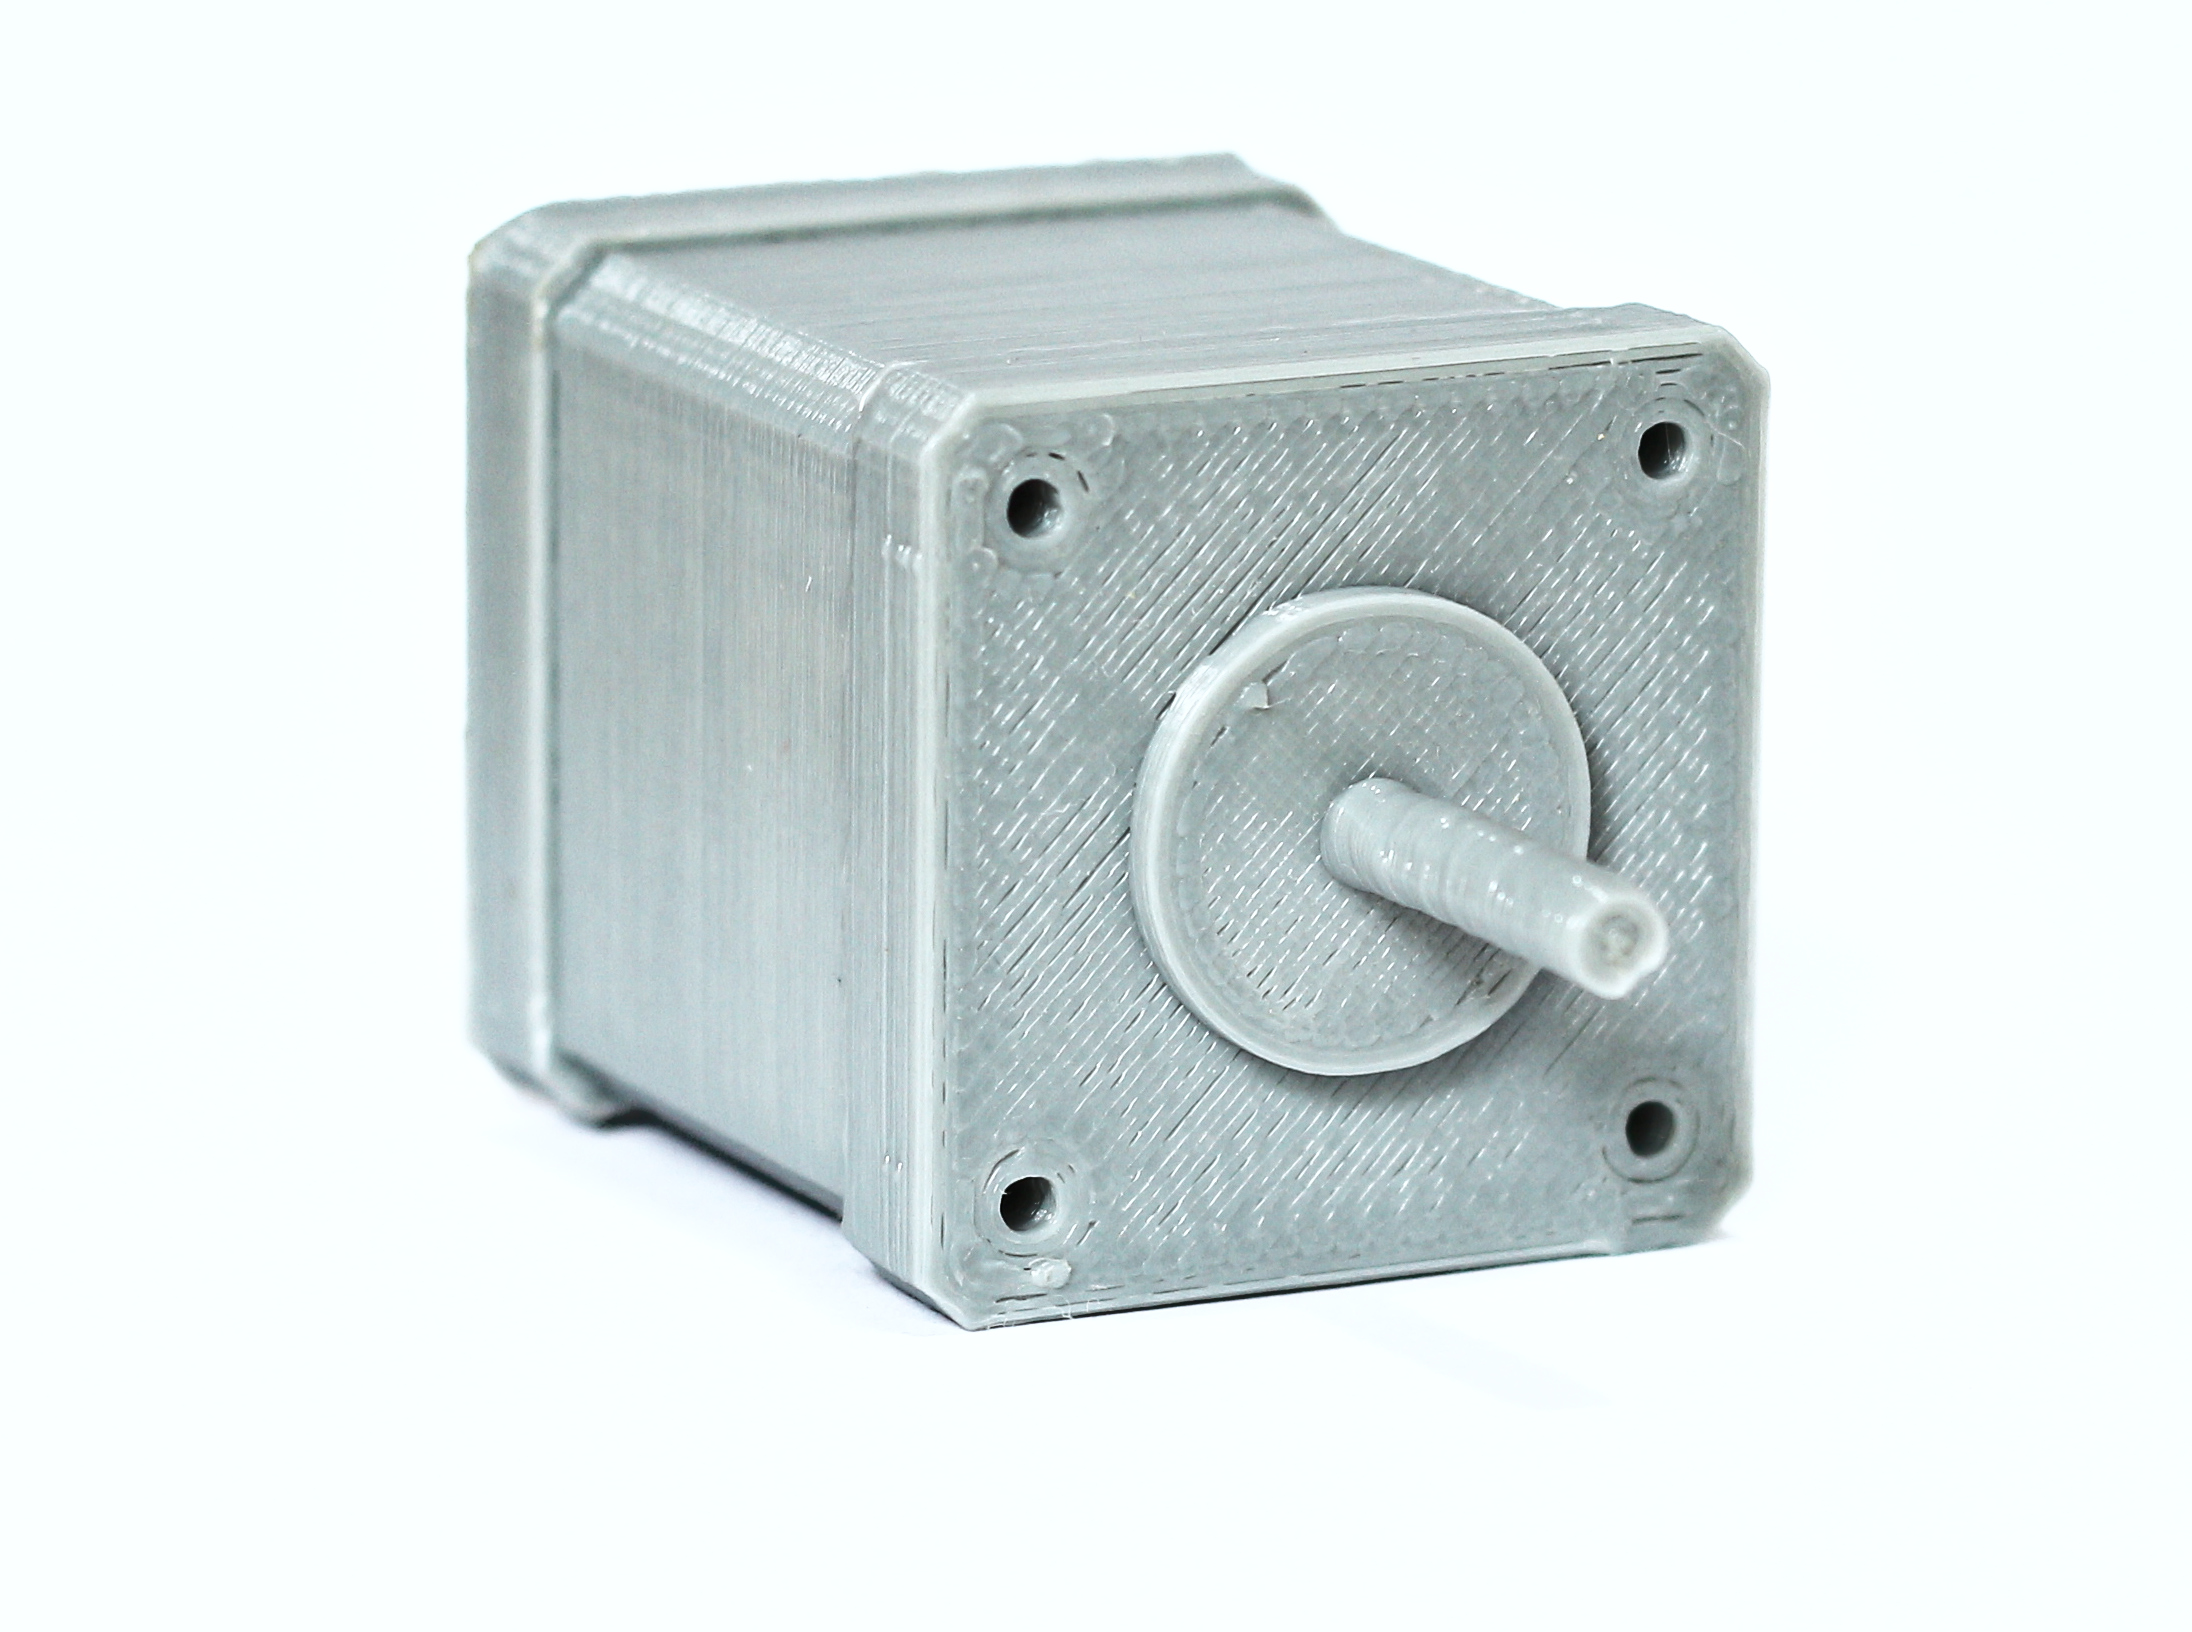
\includegraphics[width=8cm]{Img/Desarrollo/impresion3d.jpg}
    \centering
    \caption{\footnotesize{Ejemplo de fabricación digital con impresora 3D.}}
     \label{fig:impresion3d}
\end{figure}

\begin{itemize}
\textbf{A2. Parámetros}. Se sitúa en la parte inferior izquierda. Tiene los siguientes componentes:\\
        \item \textbf{- Parámetros de control}.
        Estos campos se configuran previamente mediante código en el componente B (la flecha en la figura \ref{fig:cocada2} indica la relación con el código que genera el campo).\\
        \item \textbf{- Modo Automático}. Permite visualizar automáticamente los cambios, ya sea modificando los parámetros o editando el código. En caso de deshabilitar la opción, los cambios son manuales mediante el botón de la izquierda (útil para modelos con gran cantidad de polígonos). \\
        \item \textbf{- Reiniciar parámetros}. Permite volver los campos de los parámetros al valor por defecto especificado en el código.\\
        
\end{itemize}


\end{itemize}


\begin{itemize}
\item \textbf{B. Componente Editor de código}.

\begin{itemize}
Se sitúa en la parte central del layout y es visible únicamente por el usuario Persona B (diseñador, establecido en la sección \ref{personas}).\\
CoCADa permite editar código javascript en la web con capacidad de resaltado de sintaxis mediante el editor \textbf{Ace Editor}\footnote{\url{https://ace.c9.io/}}. \\Si la opción de ``actualizar automáticamente'' se encuentra habilitada, el código se ejecuta de forma automática. De lo contrario es necesario ejecutar el programa mediante las teclas shift + enter.\\ 
Un script OpenJSCAD debe tener al menos una función definida, la funcion \textit{main()}, que retorna un objeto CSG o un vector (array) de dos o más objetos CSG. 
A continuación se analiza un programa que genera un objeto 3D mediante una operación booleana y transformaciones geométricas. En el código se puede apreciar el uso de una función ordinaria de javascript para calcular un radio, transformaciones sobre los cilindros (rotación), una operación booleana (diferencia) entre una esfera y los tres cilindros; y la definición de parámetros para el usuario. El resultado del script se puede ver  en la figura \ref{fig:jopen}.\\

\end{itemize}

\begin{minted}[baselinestretch=1, bgcolor=white, linenos, fontsize=\footnotesize]{js}

function radiusFromDiameter (d) {// Función de javascript
  return d / 2;
}

function rotcy (rot, r, h) {// Función para rotar los cilindros
  return rotate(rot, cylinder({r: r, h: h, center: true}));
}

function esferaHuecos (params) {
  var size = params.size;
  var hole = params.hole;
  var radius = radiusFromDiameter(hole);
  var height = radiusFromDiameter(size * 2.5);
  // Operación booleana: diferencia entre una esfera y 3 cilindros
  return difference(
    sphere({r: radiusFromDiameter(size)}),
    rotcy([0, 0, 0], radius, height),
    rotcy([90, 0, 0], radius, height),
    rotcy([0, 90, 0], radius, height)
  );
}

function main (params) {
  return esferaHuecos(params);
}

function getParameterDefinitions () { // Parámetros
  return [ { name: 'size', caption: 'Tamaño Esfera:', 
  type: 'slider', initial: 30, min: 5, max: 100, step: 1 },
    { name: 'hole', caption: 'Tamaño Huecos:',
    type: 'slider', initial: 10, min: 5, max: 50, step: 1 } ];
}

\end{minted}

\begin{figure}[h]
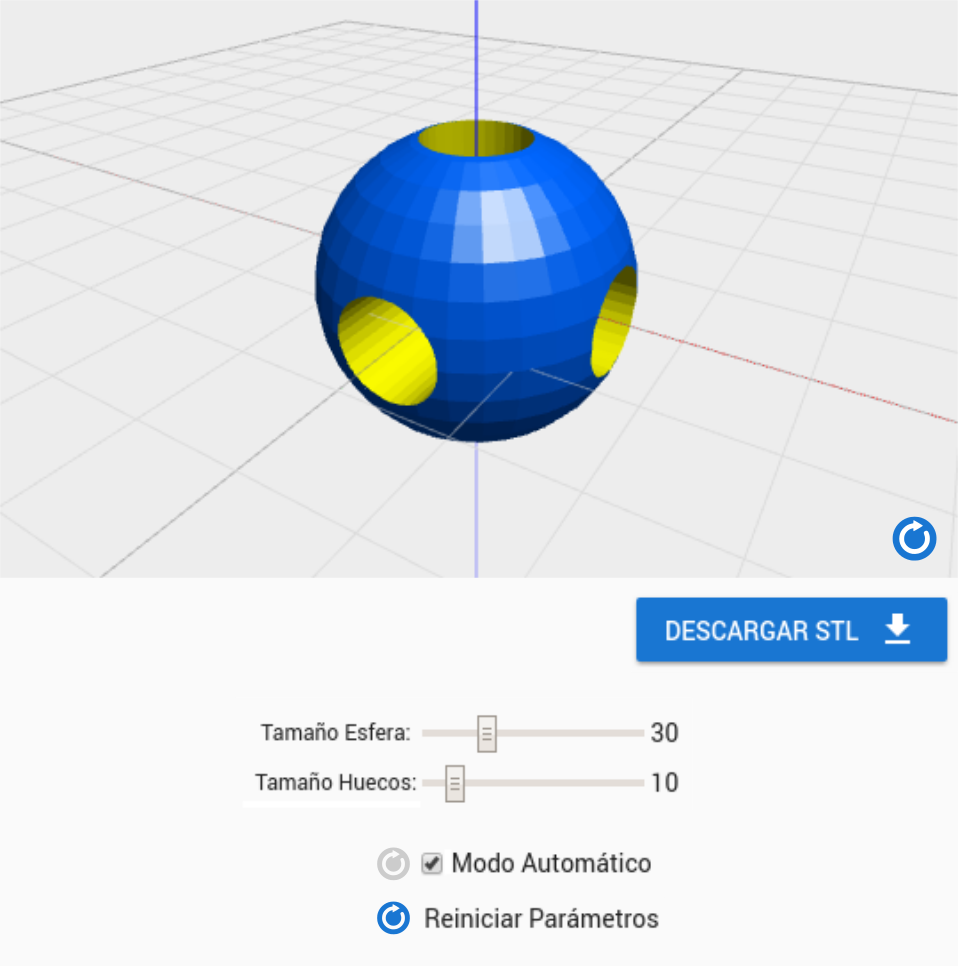
\includegraphics[width=7cm]{Img/Desarrollo/esfera-cocada.png}
\centering
\caption{\footnotesize{Modelo 3D resultante de la operación booleana (diferencia) entre una esfera y tres cilindros transformados. En la parte inferior se pueden apreciar los parámetros definidos en el código.}}
\label{fig:jopen}
\end{figure}


Todas las funcionalidades de OpenJSCAD y ejemplos de código se puede estudiar en la guía oficial\footnote{\url{https://openjscad.org/dokuwiki/doku.php}}.


\item \textbf{- Nueva Versión}. Genera una nueva versión del espacio de trabajo (Producto) y luego está disponible en el historial de versiones en el componente (D). El código versionado toma como base los parámetros modificados. 



\end{itemize}


\begin{itemize}
\item \textbf{C. Componente Compartir modelo}.
\begin{itemize}
 Se sitúa en la parte superior derecha de la pantalla. Se comparte un enlace web a una pantalla con visor reducido con el modelo. El objetivo es poder mostrar un diseño a usuarios anónimos.
\end{itemize}

\end{itemize}



\begin{itemize}
\item \textbf{D. Componente de Comentarios e Historial de modelos}.

\begin{figure}[ht]
    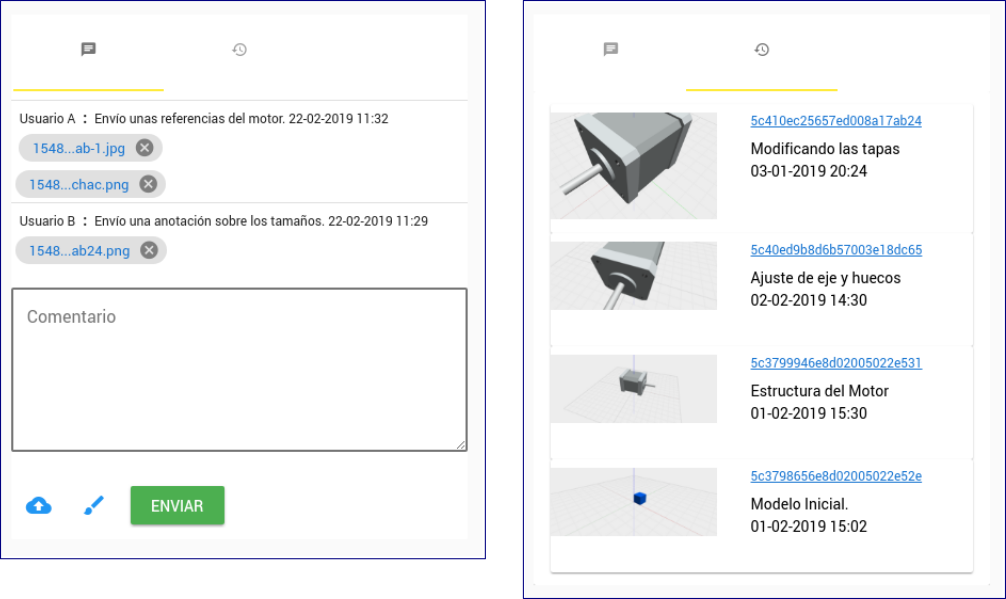
\includegraphics[width=14cm]{Img/Desarrollo/comentario00.png}
    \centering
    \caption{\footnotesize{CoCADa. Pestaña de Comentarios: formulario para carga de comentarios en un producto (izquierda). Pestaña de Historial: Listado de productos o versiones (derecha).}}
    \label{fig:comment0}
\end{figure}

\begin{itemize}
 Se sitúa en la parte inferior  derecha del layout. Utiliza un mecanismo de pestañas en inglés \textit{tabs} de manera que la selección de una opción oculte la otra, las opciones son ``Comentarios'' e ``Historial''.\\
 


 \textbf{- Componente de comentarios}. 
 Se accede a través de la primer pestaña o icono en forma de comentario. Su objetivo es lograr la comunicación entre los usuarios en forma de conversación o \textit{chat} (ver \ref{fig:comment0} (izquierda)).
 Existen dos maneras de utilizar imágenes en los comentarios:\\
 

\textbf{Como imagen adjunta}. \\
Presionando el icono de la esquina inferior izquierda del componente (ver figura \ref{fig:comment0} (izquierda)) es posible explorar archivos del dispositivo y adjuntar una imagen. 

\textbf{Como anotaciones en el modelo}. 
\begin{figure}[h]
    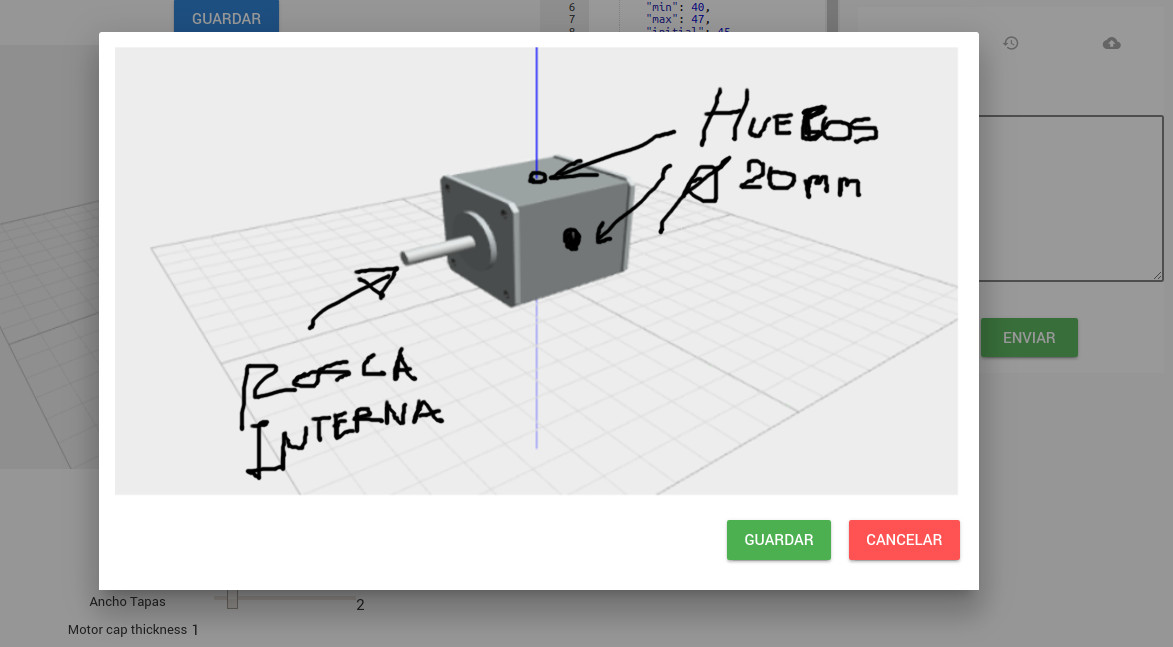
\includegraphics[width=12cm]{Img/Desarrollo/comentario2.jpg}
    \centering
    \caption{\footnotesize{ Herramienta para anotaciones sobre los modelos. Se utiliza la herramienta presionando el icono con forma de lápiz. Esto realiza una captura de pantalla del modelo y mediante una herramienta de dibujado permite hacer anotaciones sobre la imagen. Las anotaciones son muy útiles para comunicar de manera directa ideas sobre el modelo y lograr la colaboración entre participantes con diferentes competencias. }}
    \label{fig:comment2}
\end{figure}

\\




\vspace{5mm}
\textbf{- Componente de Historial}.\\
Se accede a través de la segunda pestaña o icono en forma de reloj. Permite visualizar todas las versiones o iteraciones de un producto, en orden cronológico. Una vez que se accede al producto o versión deseada, se puede modificar para generar otra versión. Esta funcionalidad es fundamental para soportar el diseño iterativo, explicado en la sección \ref{chap:cap3}. Ver figura \ref{fig:comment0} (derecha).


\end{itemize}



\end{itemize}


\clearpage
\subsection{Interacción entre Usuarios, Front-End y Back-End}

Mediante el gráfico resumido de la  arquitectura (ver figura \ref{fig:front-backend}) se pueden analizar las interacciones de los usuarios y las áreas del sistema:

\begin{figure}[ht]
    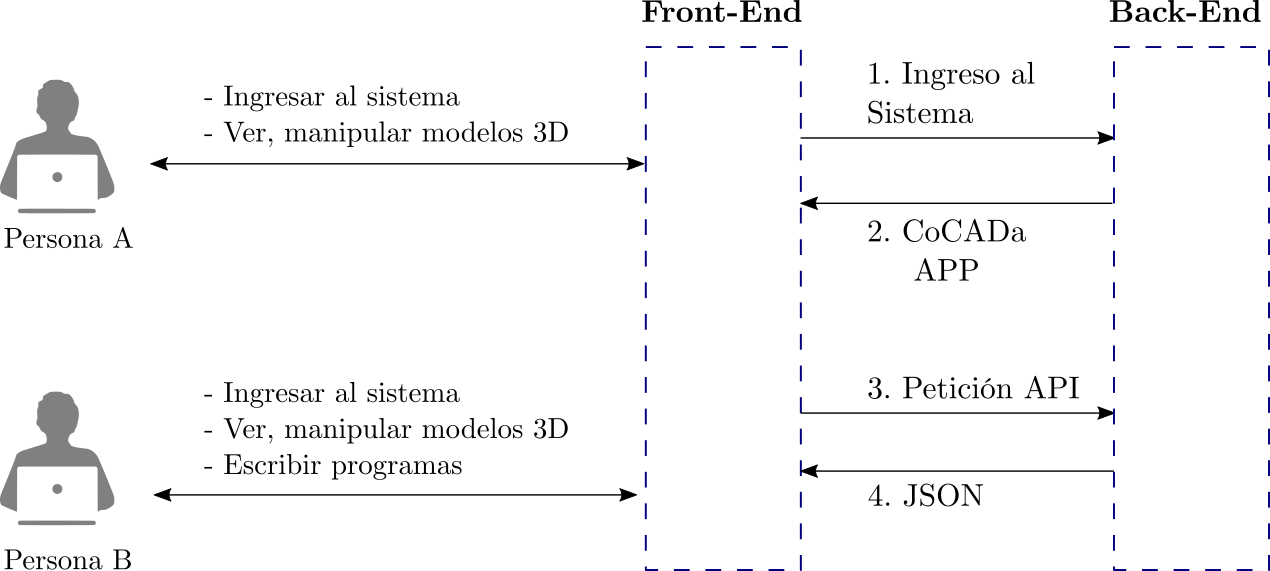
\includegraphics[width=12cm]{Img/Desarrollo/front-back.png}
    \centering
    \caption{\footnotesize{ CoCADa interacción entre usuarios, Front-End y Back-End. }}
    \label{fig:front-backend}
\end{figure}


\begin{enumerate}
    \item El usuario ingresa al sistema utilizando el navegador web (\textit{Fron-End}) mediante una URL, por ejemplo:  \url{http://cocada:3000/proyecto/000001}.
    
    \item Nuxt.js resuelve la petición en el servidor (\textit{Back-End}) según la URL ingresada por el usuario, 
    en caso de requerir recursos de la API se comunica con LoopBack. Finalmente, se genera la aplicación (CoCADa APP) con los datos solicitados y se envía al \textit{Front-End}. A partir de este momento Nuxt.js no vuelve a intervenir.  

   \item El usuario a través de CoCADa APP realiza una acción, por ejemplo: \textit{Login}, listar proyectos, ver un proyecto, generar una nueva versión, etc. El \textit{Front-End} genera la petición API correspondiente mediante Vue.js. %Tanto las acciones como las interacciones en la UI son gestionadas por Vue.js.
   
   \item LoopBack recibe la petición API, se encarga de resolver la acción y responder al \textit{Front-End} mediante documentos en formato JSON. 
   Por ejemplo: Durante el \textit{Login}, se verifica el usuario y contraseña, como respuesta se obtienen los datos de aceptación o denegación. Si la petición es la ``lista completa de los proyectos'', se retorna una colección de proyectos almacenados en la base de datos. Vue.js es el encargado de actualizar los cambios en la UI con los nuevos datos.

\end{enumerate}

